\begin{table*}[t]
  \begin{tabular}{lllp{1.0cm}p{0.8cm}lp{2.0cm}}
    Families                              &App Name             &App Website              &APK Version  &Target SDK  &Package Name              &Discovery Method                                               \\
    \midrule
    \multirow{7}{*}{Spyic}                &Cocospy              &cocospy.com              &16.3              &22                  &com.sc.cocospy.v2         &\multirow{7}{*}{\shortstack[l]{Website \\ \& \\ APK}}          \\
                                          &Minspy               &minspy.com               &16.3              &22                  &com.minspy.v3             &                                                               \\
                                          &Neatspy              &neatspy.com              &16.3              &22                  &com.sc.spyic.v3           &                                                               \\
                                          &Spyic                &spyic.com                &16.3              &22                  &com.sc.spyic.v3           &                                                               \\
                                          &Spyier               &spyier.com               &16.3              &22                  &com.sc.spyier.v2          &                                                               \\
                                          &Spyine               &spyine.com               &16.3              &22                  &com.sc.spyine.v2          &                                                               \\
                                          &Spyzie               &spyzie.io                &16.4              &22                  &com.dy.spyzie.v4          &                                                               \\
    \hline
    \multirow{5}{*}{TheTruthSpy}          &Copy9                &copy9.com                &7.85              &28                  &com.systemservice         &\multirow{5}{*}{\shortstack[l]{Website \& APK \\ \& Backend}}  \\
                                          &GuestSpy             &guestspy.com             &5.0.1             &28                  &com.systemservice         &                                                               \\
                                          &iSpyoo               &ispyoo.com               &8.80              &28                  &com.systemservice         &                                                               \\
                                          &Mxspy                &mxspy.com                &1.0               &22                  &com.mxspy                 &                                                               \\
                                          &TheTruthSpy          &thetruthspy.com          &9.41              &28                  &com.systemservice         &                                                               \\
    %\hline
    %\multirow{2}{*}{Mobile-tracker-free}  &Mobile-tracker-free  &mobile-tracker-free.com  &153               &28                  &mobile.monitor.child2021  &\multirow{2}{*}{Website}                                       \\
    %                                      &Spy24                &spy24.app                &1.0               &29                  &net.spy24.wifi            &                                                               \\
    \hline
    \multirow{2}{*}{HoverWatch}           &HoverWatch           &hoverwatch.com           &7.2.338           &28                  &com.android.core.mntw     &\multirow{2}{*}{\shortstack[l]{Website \& APK \\ \& Backend}}  \\
                                          &Snoopza              &snoopza.com              &6.1.56            &28                  &com.android.core.mngu     &                                                               \\
  \end{tabular}

  \caption{App families identified while selecting apps to study.  For
  each app in a family I show its name, website domain, APK version
  code, target SDK version, package name, and how I discovered the
  family connection.  \label{tab:apps_family}}
  \vspace*{0.1in}
\end{table*}


%\newpage
\hspace*{0.1in}\newpage
\appendix


\section{App Observations}
\label{subsec:additional_observation}

While examining the spyware apps, I observed that they
share many characteristics.  To supplement our main results, I also
describe similarities in their installation configurations and the
families of apps I discovered during our app selection process.

\subsection{Installation Configuration}
\label{subsubsec:install_configure}

Many spyware apps share common installation configurations.  These
configurations help spyware apps stay stealthy and improve
persistence. Broadly, I see the following common configurations
recommended by spyware apps: (1) turn off Google Play protection; (2)
turn off notification of the app; (3) grant various permissions (e.g.,
accessibility); and (4) disable battery optimization.  Additionally,
we note that seven apps (Clevguard, HoverWatch, iKeyMonitor, Meuspy, Spyhuman, Spy24, and TheTruthSpy) abuse accessibility to
automatically click buttons (e.g., automatically clicking on the grant permission button when the app is requesting MediaProjection permission), a
behavior much like that of malware. Finally, I find that three apps
(Meuspy, Mobile-tracker-free, and Spy24) use a loader app to install
the actual app, and a loader facilitates the installation process of the two apps (Meuspy and Spy24) that do not have a launcher activity (as mentioned in Section~\ref{subsubsec:hide_icon}).

\subsection{App Family}
\label{subsubsec:app_family}

In the process of selecting the 14 apps in our study, I identified
various families of apps that are connected: apps
that are rebranded versions of others.  Table~\ref{tab:apps_family} lists the
three families of apps I observed. The families I identify echo what is documented by
other industry reports~\cite{Tekstalk86:online,
esetandr4:online}. I name each family using the name
of the app whose website domain has the highest Tranco ranking, as shown in
Table~\ref{tab:apps_selected}.

Spyic is the largest family I find, consisting of seven variants.
After examining their APKs, I conclude that all apps in this family
are rebranded versions of each other with different package names.  We
note that websites used by these apps all include a CSS file
(\texttt{alicdn.com/t/font\_xxx.css}) hosted at Alicdn (a Chinese
CDN), and some of the debug strings are in Chinese.
While it is likely that this family of apps is operated
by a Chinese-speaking group, it does not seem to operate in China and
does not offer Chinese as a language option on its website,
potentially due to legal concerns.

TheTruthSpy family includes five apps: Copy9, GuestSpy, Mxspy, iSpyoo
and TheTruthSpy. Examining the APKs of Copy9 and GuestSpy suggests that
they are simply rebranded versions of TheTruthSpy. Mxspy uses the same
backend as Copy9.  Snoopza is a rebranded version of HoverWatch, which
can be determined by examining its APK (similar code), backend (same
infrastructure) and website (generated with the same
template).

I also note that Spy24 advocates for Mobile-tracker-free on its
website. However, I observe that the two apps are very different in
their implementation, and I include both of them in our study.

I end by noting that this list is not comprehensive.  When investigating apps
to study, our primarily goal was to filter out duplicate apps that are
likely rebranded versions of others to avoid redundant work and
results.  Classifying apps more systematically and comprehensively is
a research area in itself~\cite{SuarezTangil2013Dendroid,
Zhang2014Semantics, deshotels2014droidlegacy, pierazzi2020data}.

%% I conclude by noting two things. First, I are not trying to
%% comprehensively list families of apps that are in the wild in
%% Table~\ref{tab:apps_family}. Instead, I only list apps that were
%% considered by us. Second, our main goal was to filter out duplicate
%% apps that are likely rebranded versions of others, and classifying an
%% app into a specific family was not our focus (it is a research area in
%% itself~\cite{SuarezTangil2013Dendroid, Zhang2014Semantics,
%% deshotels2014droidlegacy, pierazzi2020data}).

\newcommand{\hash}[1]{\texttt{#1}}

\begin{table*}[t]
  \begin{tabular}{lll}
    App Name  & APK Version & SHA-1 Hash of the APK \\
%    App Name\hspace*{0.6in}\hfill             &APK Version Code\hspace*{0.2in}\hfill   &SHA-1 Hash of the APK                         \\
    \midrule
    mSPY                 &6.3.2             & \hash{4e675734487baaa93533f5c187c376d37ce28eb3}  \\
    Mobile-tracker-free  &153               & \hash{e18637c9576a295b02ab3dc8282eb4ca242942dd}  \\
    Clevguard            &4.0.7             & \hash{e8234174971f4c50964f8b12987f1fa6ce47699a}  \\
    \ltgrey HoverWatch   &7.2.338           & \hash{33c12f3fbe2b510ceb3111f8198f974040ab05ba}  \\
    \ltgrey Flexispy     &4.16.1            & \hash{07786dc314f8cab968d0c5a310a71601543bea0e}  \\
    \ltgrey Spyic        &16.3              & \hash{37ea4d27e3ac25c48b72d99c1503e56853ce7260}  \\
    Spyhuman             &311               & \hash{f567eff3134b04c0efbc14fa6bc4916bb851ae0c}  \\
    TheTruthSpy          &9.41              & \hash{d421e9a94c742f80e9ff573b73576eaf1bb8dc25} \\
    iKeyMonitor          &9.8               & \hash{2f6f807f2ac1b5a423e006a667db15c3f7229c6d}  \\
    \ltgrey Cerberus     &3.6.9             & \hash{40345be0287e47224d951cd3644ac0bd7f49e150}  \\
    \ltgrey Spy24        &1.0               & \hash{324fb89cec42ab67be6b644b62522c89711b53b0}  \\
    \ltgrey Spapp        &16.6              & \hash{7936fa6cf35cf74b5e156d63849188c28de86d0b}  \\
    Meuspy               &5.20              & \hash{2eb5bc667a499e44d3c77c9f16c23d278e56e9f7}  \\
    Highstermobile       &3.26              & \hash{c0d6b1a18a8cc49f7f804451ee992fe0670072ec}  \\
  \end{tabular}
  \caption{The APK's version code and SHA-1 hash of the apps I study.
Shading added to improve readability.
  \label{tab:add_app_info}}
  \vspace*{0.1in}
\end{table*}


\section{Code Obfuscation}
\label{sec:apk_obfuscation}

After decompiling all the APKs with \texttt{JADX} and examining the
decompiled Java code, I observed that two apps (Highstermobile and
iKeyMonitor) did not protect their code with obfuscation
(i.e., the names of classes, fields, and methods are preserved). Nine
apps obfuscated the names of classes, fields, and methods, which could
be done easily with tools such as ProGuard~\cite{LeaderIn1:online}.
The last three (Meuspy, SPAPP, and Spyhuman)
went a step further and also obfuscated strings (potentially to hinder
reverse engineering efforts). Among these three, Meuspy used
\texttt{paranoid} (an open source string obfuscation
tool~\cite{MichaelR90:online}), and I deobfuscated their strings with
an open source \texttt{paranoid}
deobfuscator~\cite{giacomof39:online}. I wrote our own deobfuscators
for SPAPP and Spyhuman.


\section{Additional Figures and Tables}
\label{sec:additional_figures}

Table~\ref{tab:add_app_info} shows the list of spyware of apps I chose, their APK version code, and the SHA-1 hash for the corresponding APK I study.
Figure~\ref{fig:da} shows an example of an app disabling both the Force Stop and Uninstall buttons on a phone running Android 6.

%% forces Fig 3 to be placed into the second column
\vspace*{2in}
\hspace*{1in}

\begin{figure}[t]
\centering
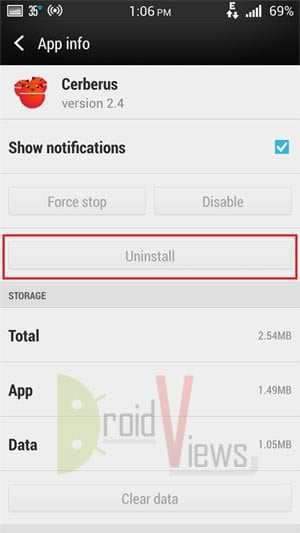
\includegraphics[width=0.8\columnwidth]{fig/DA.pdf}
\caption{An example of an app disabling both the
Force Stop and Uninstall buttons on Android 6.}
\label{fig:da}
\end{figure}
